\subsection{Pregunta a): Función de cálculo de la TVI}

Implementar una función que, dada la línea fallada, entregue las barras con TVI distinta de cero y su valor.

\subsubsection{Metodología}

La función \texttt{calcular\_TVI} se implementó en Python sobre la interfaz de programación de PowerFactory. Recibe como entradas el objeto \texttt{app} y un \textit{string} con el nombre de la línea fallada. Su salida es una lista de listas con una entrada por cada barra cuya TVI es distinta de cero:

\begin{center}
\fbox{\texttt{[[nombre\_barra, TVI], [nombre\_barra, TVI], ...]}}
\end{center}

Si ninguna barra viola la envolvente, la función retorna una lista vacía, y si la simulación no converge retorna \texttt{False}. Este resultado es el criterio que se utilizará en la Pregunta d) para verificar que la compensación es suficiente.

Para cada contingencia, la función ejecuta la siguiente secuencia:

\begin{enumerate}
    \item \textbf{Preparación de los eventos de simulación.} Se reutilizan el evento de cortocircuito (\texttt{ShcLineEvent}) y el de interruptor (\texttt{TripLineEvent}) del caso de estudio, apuntando a la línea fallada, y cualquier otro evento queda fuera de servicio, de modo que no se acumulen fallas de corridas anteriores.
    \item Cortocircuito trifásico franco (resistencia y reactancia nulas) al $50$\,\% de la línea en $t = 0$ s.
    \item Desconexión de la línea en $t = 0{,}1$ s (despeje a los 100 ms), mediante un evento de simulación y no modificando el estado de la línea en el caso de estudio, de modo que las contingencias siguientes no se simulen con una línea menos.
    \item Cálculo de las condiciones iniciales y ejecución de la simulación RMS hasta $t = 20$ s.
    \item Extracción de la magnitud de tensión en p.u. de las 39 barras desde el archivo de resultados.
    \item Construcción de las envolventes según \cite{wildenhues}, con $\beta = 0{,}05$ y $v_{st} = 0{,}9$ p.u. (ecuaciones~\eqref{eq:tlow} y~\eqref{eq:tupp}), cálculo de la TVI de cada barra mediante las ecuaciones~\eqref{eq:tvi} y~\eqref{eq:vv}, y conservación de los valores distintos de cero.
\end{enumerate}

La integral de la ecuación~\eqref{eq:tvi} se evalúa de forma numérica mediante la regla del trapecio sobre las muestras de tensión del archivo de resultados:
\begin{equation}
    \mathrm{TVI}_i \approx \sum_{k} \frac{v_{v,k}^{(i)} + v_{v,k+1}^{(i)}}{2}\,\left(t_{k+1} - t_k\right),
\end{equation}
donde $v_{v,k}^{(i)}$ es la violación instantánea de la barra $i$ en el instante $t_k$. Como el paso de las muestras no es uniforme, se integra directamente sobre el vector de tiempos del archivo de resultados. Una barra se considera con violación solo si su TVI supera una tolerancia de $10^{-6}$ p.u.$\cdot$s, para evitar falsos positivos por ruido numérico.

\paragraph{Ventana de integración.}
La integral se evalúa desde el despeje de la falla ($t = 0{,}1$ s) hasta $t_{end} = 20$ s. Durante el cortocircuito, las barras cercanas a la falla presentan tensiones inferiores a la envolvente en todas las contingencias, por lo que incluir ese intervalo sumaría una violación que no corresponde a la recuperación posterior. Esta decisión se verificó con la contingencia Line 28 - 29: integrando desde $t = 0$ s el total fue $0{,}204$, aproximadamente el doble del valor referencial de la guía, mientras que integrando desde el despeje fue $0{,}0969$.

El código completo de la función se encuentra en el Anexo~\ref{anexo:codigo_a}.

\subsubsection{Resultados}

La Tabla~\ref{tab:salida_a} muestra la salida de la función para la contingencia Line 28 - 29, y la Tabla~\ref{tab:tvi_total_a} el valor de su TVI total, calculada como la suma de la TVI de todas las barras (ecuación~\eqref{eq:tvitot}).

\begin{table}[H]
    \centering
    \caption{Salida de \texttt{calcular\_TVI} ante la contingencia Line 28 - 29.}
    \label{tab:salida_a}
    \begin{tabular}{|l|c|}
        \hline
        Barra & TVI [p.u.$\cdot$s] \\
        \hline
        Bus 26 & 0.000197 \\
        \hline
        Bus 28 & 0.020780 \\
        \hline
        Bus 29 & 0.040256 \\
        \hline
        Bus 38 & 0.035617 \\
        \hline
    \end{tabular}
\end{table}

\begin{table}[H]
    \centering
    \caption{TVI total de la contingencia Line 28 - 29.}
    \label{tab:tvi_total_a}
    \begin{tabular}{|l|c|}
        \hline
        Contingencia & TVI total [p.u.$\cdot$s] \\
        \hline
        Line 28 - 29 & 0.096850 \\
        \hline
    \end{tabular}
\end{table}

La Figura~\ref{fig:bus29_a} ilustra el cálculo para la barra 29, la de mayor TVI en esta contingencia. Durante el cortocircuito (0 a 0.1 s) la tensión cae desde 1.05 p.u. a valores cercanos a 0.2 p.u., muy por debajo de la envolvente, por lo que ese intervalo no se considera. Tras el despeje, las áreas sombreadas entre la trayectoria y los límites de la envolvente corresponden a la TVI de la barra.

\begin{figure}[H]
    \centering
    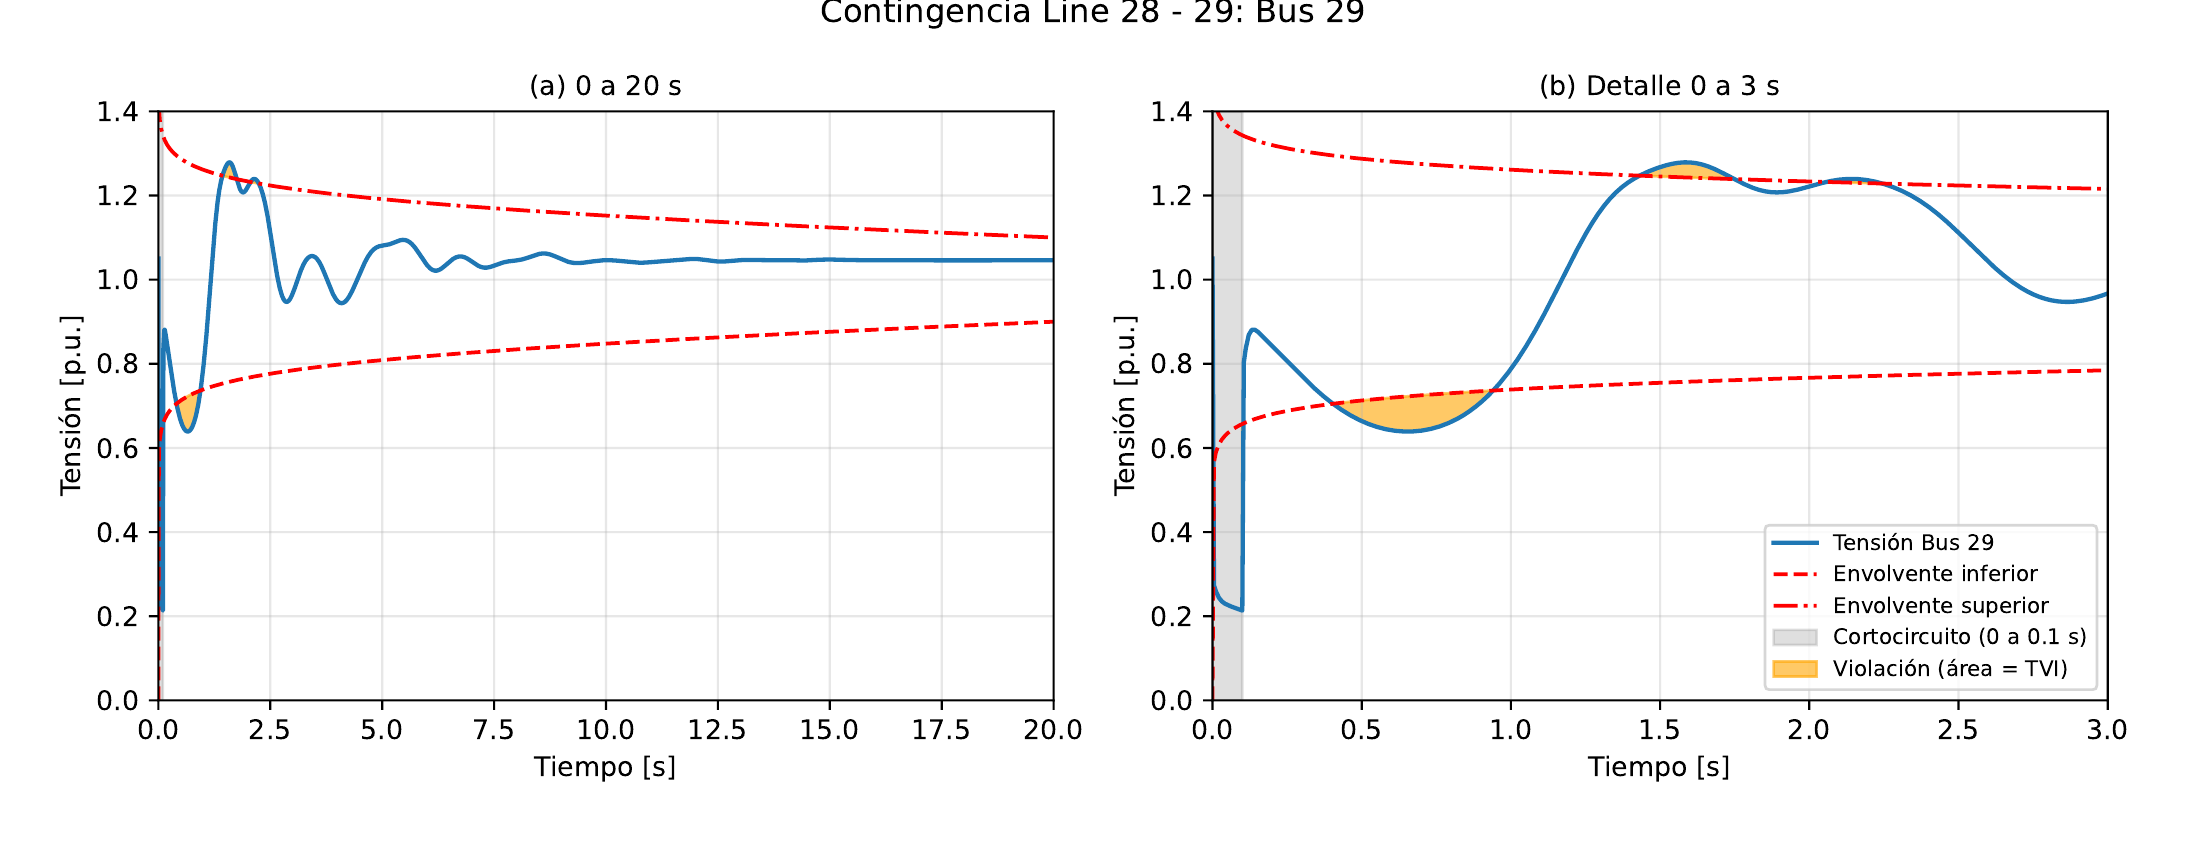
\includegraphics[width=\textwidth]{Desarrollo/Imagenes Informe/tvi_bus29_line_28_29.png}
    \caption{Trayectoria de tensión de la barra 29 y envolvente ante la contingencia Line 28 - 29: (a) vista completa y (b) detalle de los primeros 3 s. El área sombreada corresponde a la TVI de la barra.}
    \label{fig:bus29_a}
\end{figure}

Para una línea cuya contingencia no produce violaciones de la envolvente, la función retorna una lista vacía, \texttt{[]}.

\subsubsection{Comentarios}

El valor de TVI total obtenido para la contingencia Line 28 - 29 es $0{,}0969$, un $6$\,\% inferior al valor referencial de la guía ($0{,}1034$). El orden de magnitud coincide, y las diferencias menores pueden atribuirse al paso de integración de la simulación y al método de integración numérica empleado.

La mayor parte de la TVI se concentra en las barras 28 y 29, que son los terminales de la línea fallada. La barra 26 aporta un valor marginal ($0{,}000197$, cerca del $0{,}2$\,\% del total). Además aparece la barra 38, una barra de generación de 16.5 kV conectada eléctricamente a la barra 29, cuya tensión acompaña la de esta última.

Para que cada contingencia se simule de forma independiente, la función no acumula eventos de corridas previas y abre la línea mediante un evento de simulación. Además, solo conserva las barras con TVI distinta de cero. Esto permite usar directamente el largo de la lista de salida como criterio de factibilidad en la Pregunta d): una lista vacía indica que ninguna barra viola la envolvente.

Una simulación completa de una contingencia tarda aproximadamente 5 s: 0.9 s en el cálculo de condiciones iniciales, 0.6 s en la simulación RMS y 3.4 s en la lectura de resultados. Este valor es relevante para planificar el número de evaluaciones de la optimización de la Pregunta d).